\documentclass{article}

% PACKAGES
\usepackage[utf8]{inputenc}
\usepackage{graphicx}
\usepackage{amsmath}
\usepackage[hyphens]{url}
\usepackage[a4paper, margin=2.5cm]{geometry} % Adjusted margins for single column
\usepackage{caption}
\usepackage{float} % Required for the [H] figure placement option
\usepackage{hyperref}

\hypersetup{
    colorlinks=true,
    linkcolor=blue,
    filecolor=magenta,
    urlcolor=cyan,
}

% DOCUMENT INFORMATION
\title{\textbf{A Proof-of-Concept for Automatic Facet Discovery in E-Commerce Search}}
\author{Rauf Aliev}
\date{June 2017 (Updated September 2025)}

\begin{document}

    \maketitle

    \begin{abstract}
        This paper addresses a significant challenge in e-commerce information retrieval: the failure of standard keyword search systems to correctly interpret complex user queries that contain product attributes. Queries such as "blue XL Burton jacket" are often processed as a simple set of keywords, leading to irrelevant results and compelling users to engage in a laborious manual filtering process. We present a proof-of-concept (PoC) for an automatic facet discovery system designed to parse user queries, identify terms corresponding to product facets (e.g., color, brand, size), and apply these filters automatically. This research demonstrates a practical methodology for bridging the semantic gap between unstructured free-text search and structured faceted navigation, thereby enhancing result relevance and improving the overall user experience.
    \end{abstract}

    \section{Introduction}

    Faceted search is an integral feature of modern e-commerce platforms, fundamentally improving the user's search and discovery experience. From a user-centric perspective, faceted navigation decomposes search results into multiple, orthogonal categories (facets), each with corresponding value counts. This paradigm enables users to iteratively refine, or "drill down," into the result set by applying filters in any desired sequence.

    The utility of this functionality is particularly evident when interacting with large-scale product catalogs, as it substantially improves product findability, mitigates user frustration, and provides a structured navigational framework. Furthermore, faceted search architectures programmatically generate relevant landing pages for long-tail keyword queries, a long-standing strategy in search engine optimization that was traditionally accomplished through static category pages. A video demonstration of the system is available online\footnote{\url{https://player.vimeo.com/video/223100657}}.

    \section{A Taxonomy of User Search Queries}

    Empirical research from the Baymard Institute classifies user search behavior into 12 distinct query types, the majority of which are inadequately supported by out-of-the-box e-commerce search engines. These types are:

    \begin{enumerate}
        \item \textbf{Exact Searches}: Queries for specific products via title or model number (e.g., \textit{Keurig K45}).
        \item \textbf{Product Type Searches}: Broad queries for product categories (e.g., \textit{Sandals}).
        \item \textbf{Symptom Searches}: Problem-based queries where the user seeks a product as a solution (e.g., \textit{“stained rug”}).
        \item \textbf{Non-Product Searches}: Informational queries regarding policies or company details.
        \item \textbf{Feature Searches}: Queries specifying particular product attributes (e.g., \textit{Waterproof cameras}).
        \item \textbf{Thematic Searches}: Queries for abstract or conceptual categories (e.g., \textit{“Living room rug”}).
        \item \textbf{Relational Searches}: Queries based on a product's association with another entity (e.g., \textit{Movies starring Tom Hanks}).
        \item \textbf{Compatibility Searches}: Queries for products compatible with another item (e.g., \textit{Lenses for Nikon D7000}).
        \item \textbf{Subjective Searches}: Queries using non-objective, qualitative terms (e.g., \textit{“High-quality kettles”}).
        \item \textbf{Slang, Abbreviation, and Symbol Searches}: Queries employing linguistic shortcuts (e.g., \textit{Sleeping bag -10 deg}).
        \item \textbf{Implicit Searches}: Queries that omit context-dependent qualifiers.
        \item \textbf{Natural Language Searches}: Queries formulated in complete sentences.
    \end{enumerate}

    \begin{figure}[H]
        \centering
        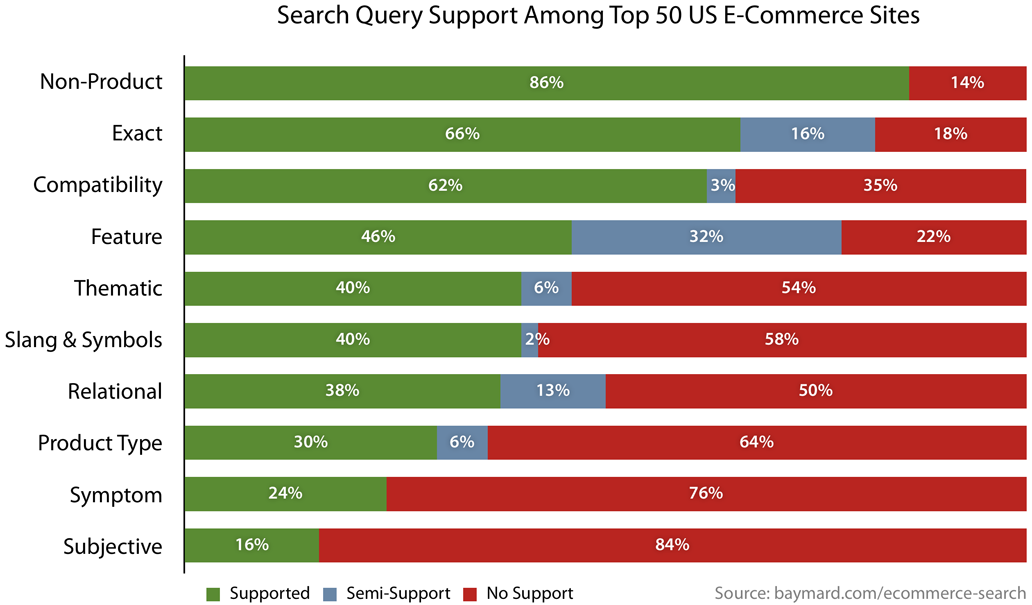
\includegraphics[width=\columnwidth]{ecommerce-search-01-query-support-e26a0c0f33559b8702edfe2f626a3dba-1.png}
        \caption{A chart from Baymard.com illustrating the poor support for various e-commerce search query types.}
        \label{fig:baymard_chart}
    \end{figure}

    While platforms such as SAP Commerce provide foundational support for some of these types, the implementation often lacks the necessary sophistication for accurate intent interpretation. Neither the platform nor its underlying SOLR search engine can natively associate query terms with semantic concepts. The proposed PoC serves as a semantic bridge between these free-text queries and the platform's powerful faceted search capabilities.

    \section{The Challenge with Conventional Faceted Search}

    Conventional faceted search implementations present known usability challenges. Although platforms display facets relevant to an initial query, the presence of attribute-related terms within the query itself can paradoxically cause those same facets to be excluded from the results. For instance, in the query “blue armada jacket XXL,” a standard search engine processes all four terms as a free-text request, returning only documents containing all four keywords.

    This approach is fundamentally flawed and leads to a cumbersome, multi-step user journey.

    \begin{figure}[H]
        \centering
        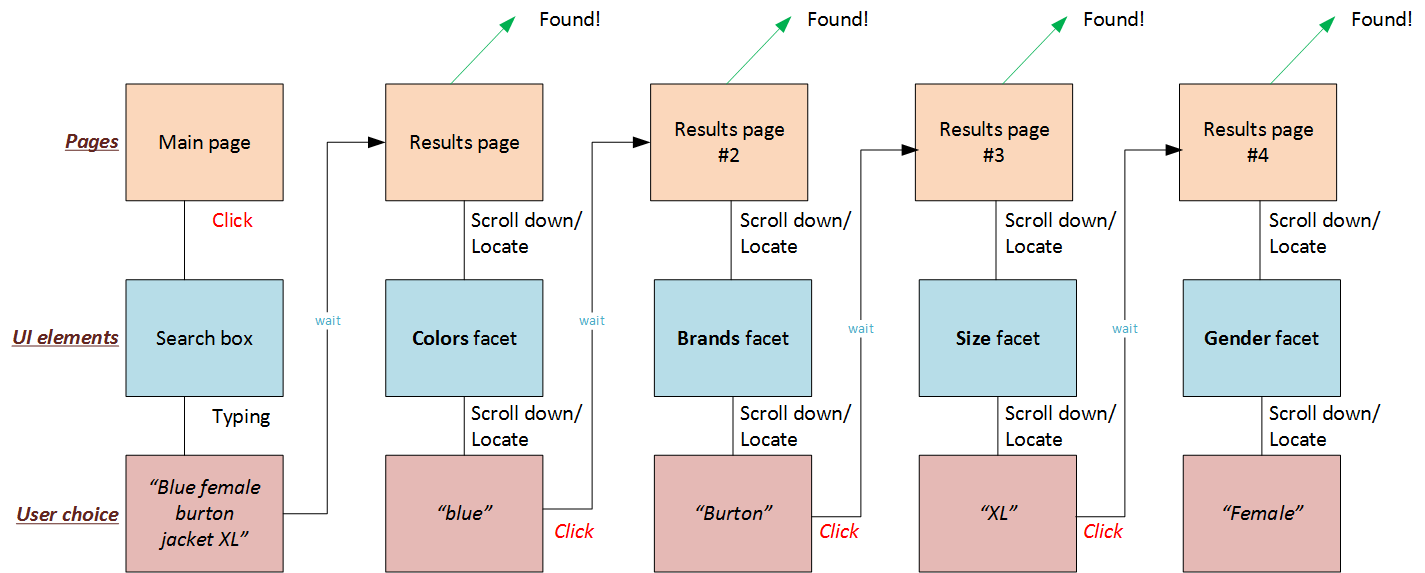
\includegraphics[width=\columnwidth]{searchimproved10.png}
        \caption{A typical e-commerce interface showing multiple facet categories on a sidebar, which users must manually interact with to refine search results.}
        \label{fig:facet_ui}
    \end{figure}

    A default SAP Commerce implementation, for example, yields highly irrelevant results for the query “blue female XL Burton jacket”.

    \begin{figure}[H]
        \centering
        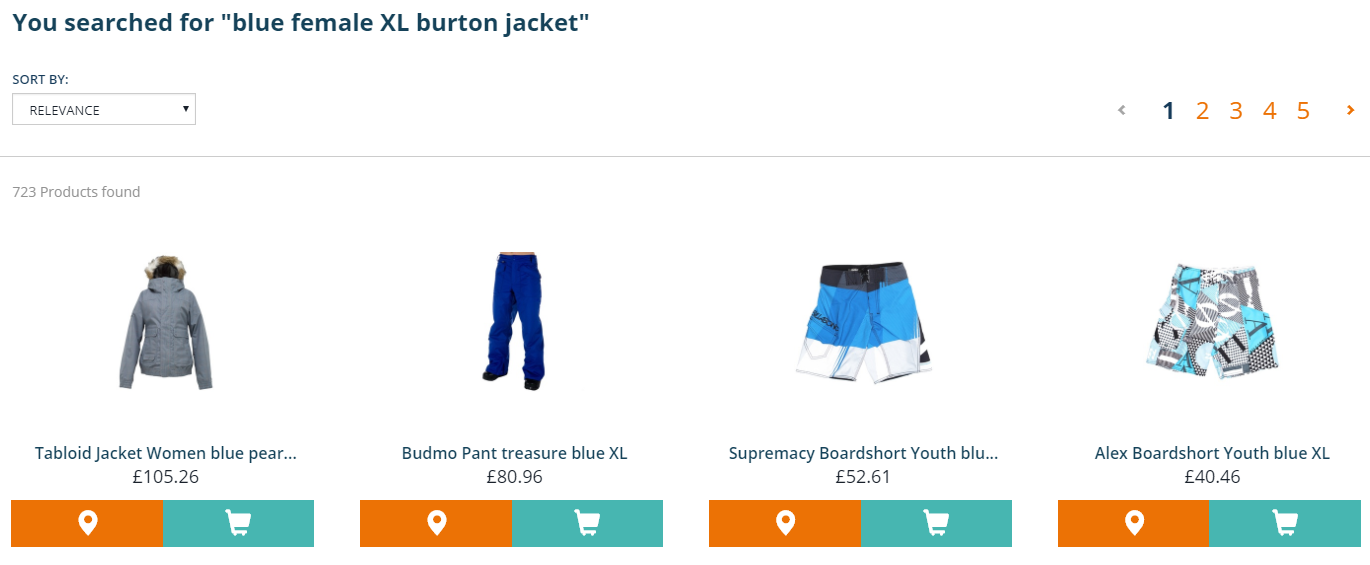
\includegraphics[width=\columnwidth]{2017-06-25_21h36_23-1.png}
        \caption{Standard SAP Commerce Cloud search results for “blue female XL Burton jacket”, showing irrelevant products.}
        \label{fig:default_apparel}
    \end{figure}

    The results include items that are not jackets, not blue, not for women, and mostly not from the specified brand. In contrast, the proposed PoC delivers highly relevant results for the identical query.

    \begin{figure}[H]
        \centering
        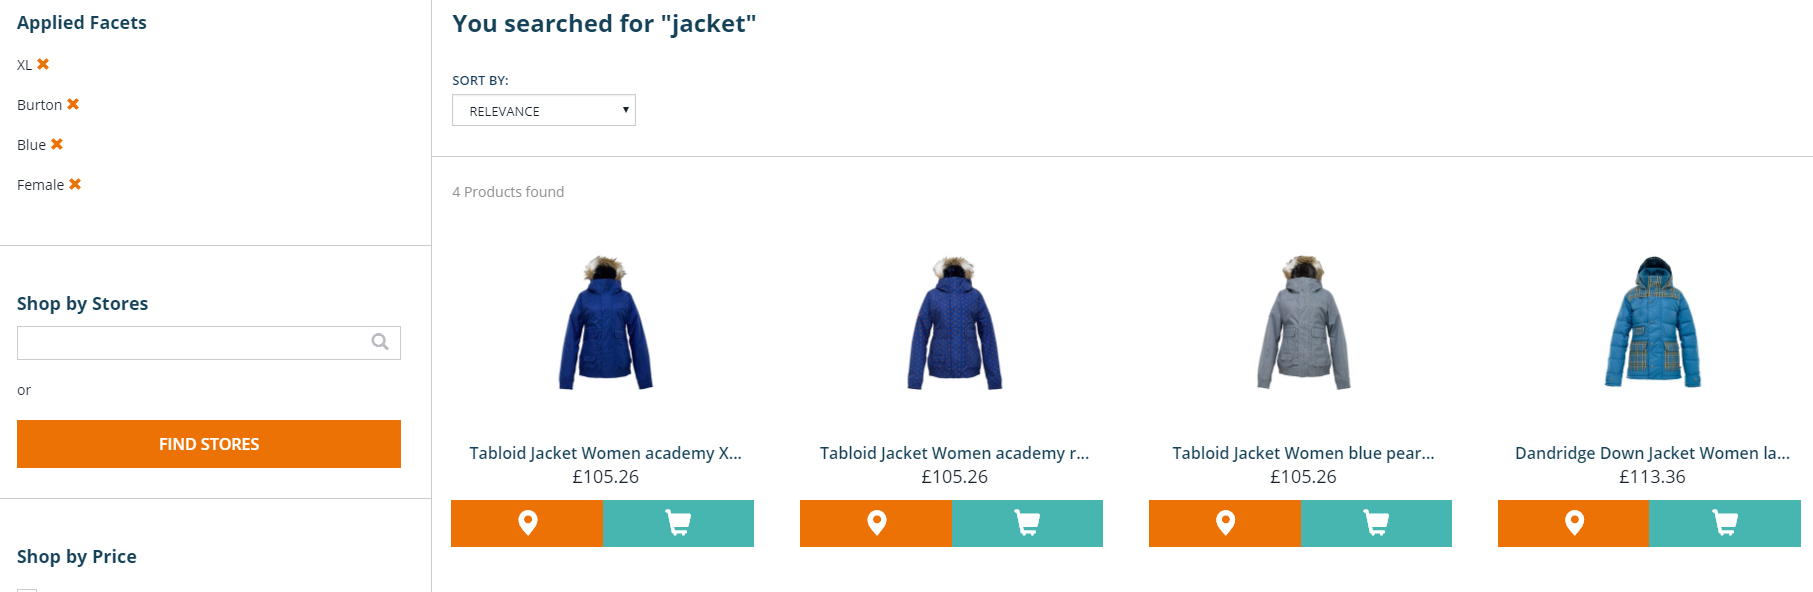
\includegraphics[width=\columnwidth]{2017-06-25_21h39_15-1.png}
        \caption{PoC results for the identical query, showing correctly filtered, relevant products.}
        \label{fig:poc_apparel}
    \end{figure}

    This performance improvement is consistent across different product domains. For an electronics catalog, the query “fixed camera lenses from canon” on a standard system yields irrelevant products.

    \begin{figure}[H]
        \centering
        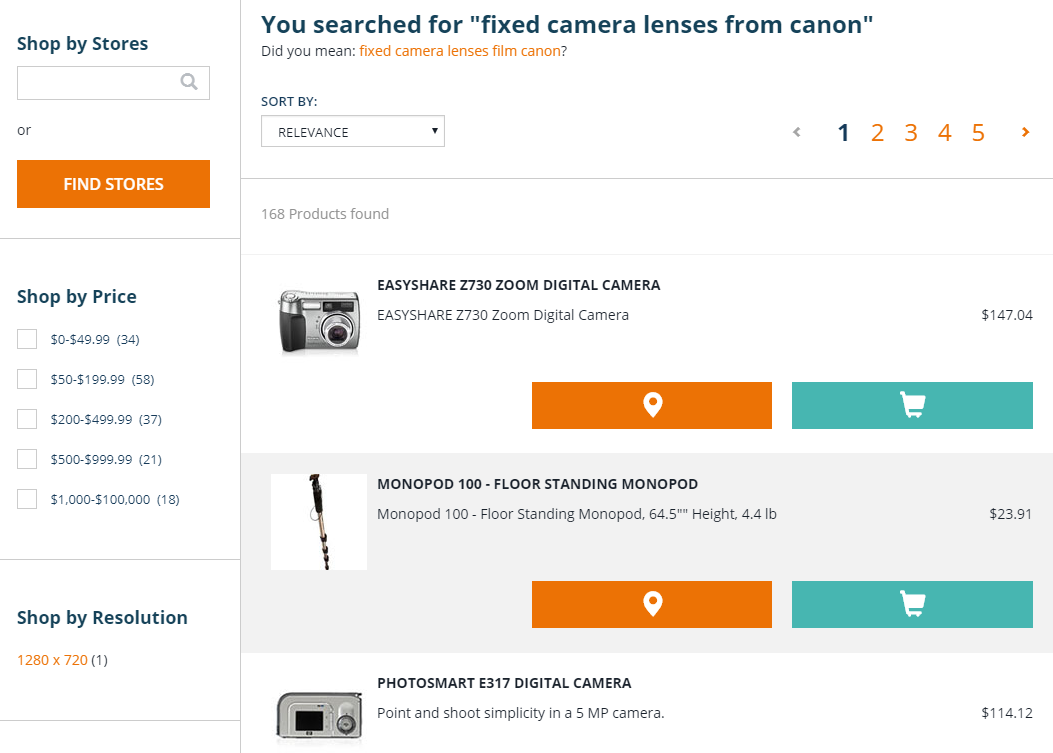
\includegraphics[width=\columnwidth]{2017-06-25_21h45_27-1.png}
        \caption{Standard search performance for “Fixed camera lens from Canon”.}
        \label{fig:default_electronics}
    \end{figure}

    The proposed system, however, correctly identifies and filters for the requested products.

    \begin{figure}[H]
        \centering
        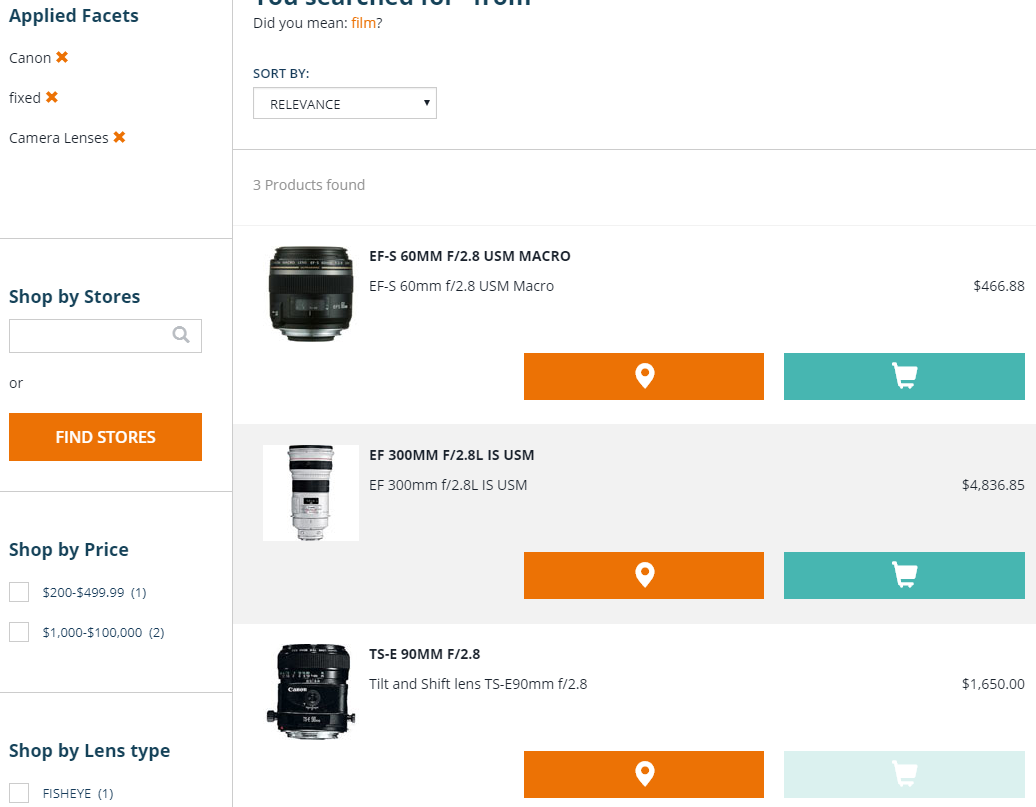
\includegraphics[width=\columnwidth]{2017-06-25_21h47_181-1.png}
        \caption{PoC performance for “Fixed camera lens from Canon”.}
        \label{fig:poc_electronics}
    \end{figure}

    The system can also interpret numerical ranges, correctly applying a filter for the "5-5.9 Mp" facet range for a query like “5 mp kodak camera”.

    \begin{figure}[H]
        \centering
        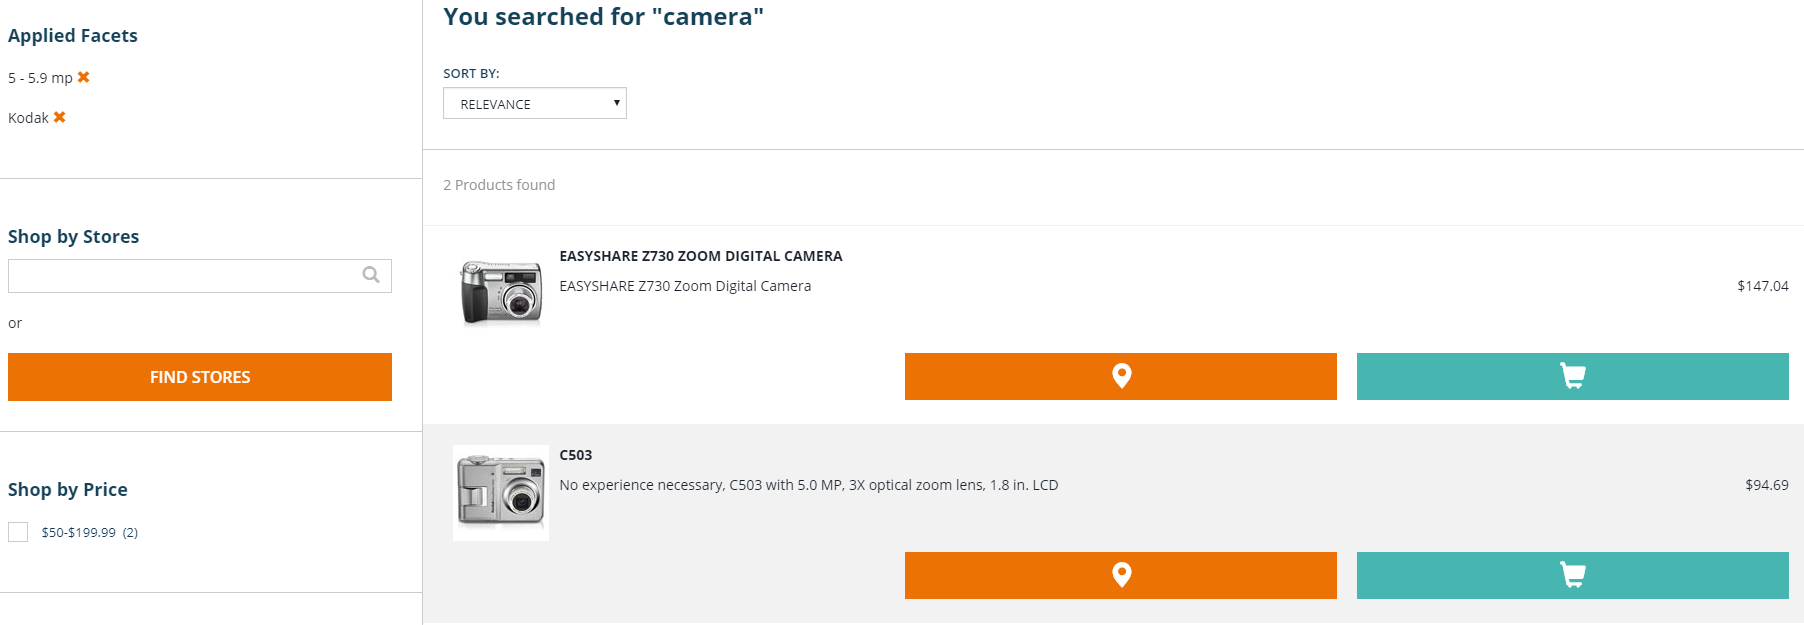
\includegraphics[width=\columnwidth]{2017-06-25_21h54_03.png}
        \caption{The PoC applying a facet range for the query “5 Mp Kodak camera”.}
        \label{fig:poc_range}
    \end{figure}

    \section{Implementation Strategy}

    While the PoC implements fully automatic query interpretation, a production deployment would benefit from A/B testing to determine the optimal strategy. An alternative, non-automatic approach involves presenting the interpreted query as a one-click suggestion alongside the standard keyword search results.

    \begin{figure}[H]
        \centering
        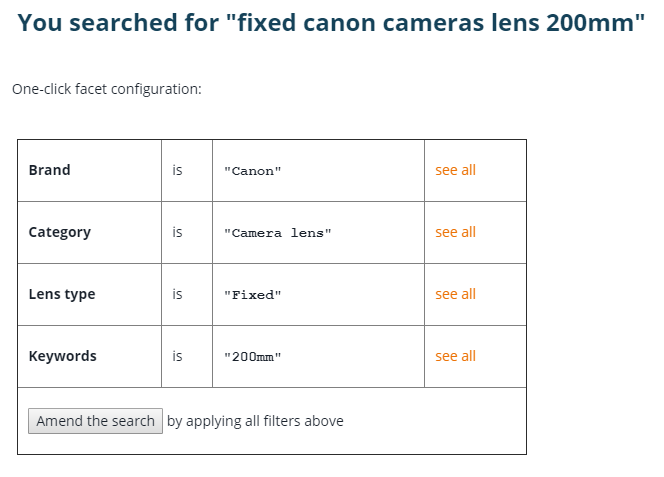
\includegraphics[width=0.8\columnwidth]{2017-06-26_02h13_24-1.png}
        \caption{A conceptual mockup of a search suggestion panel as an alternative to fully automatic interpretation.}
        \label{fig:suggestion_mockup}
    \end{figure}

    \section{Technical Architecture}

    The system's architecture is depicted below. It operates by analyzing the input query to extract terms that correspond to known facet values.

    \begin{figure}[H]
        \centering
        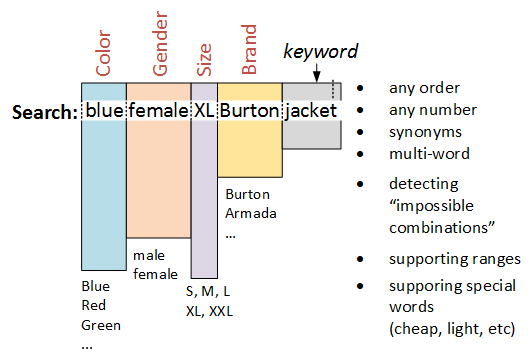
\includegraphics[width=0.6\columnwidth]{searchimproved30.png}
        \caption{High-level system architecture for the automatic facet discovery system.}
        \label{fig:architecture}
    \end{figure}

    A primary technical challenge is resolving ambiguity. For example, the query “\textit{Canon flash memory}” is ambiguous if the product catalog contains no flash memory manufactured by Canon. This ambiguity is resolved when the catalog contains products that satisfy all specified attributes.

    \begin{figure}[H]
        \centering
        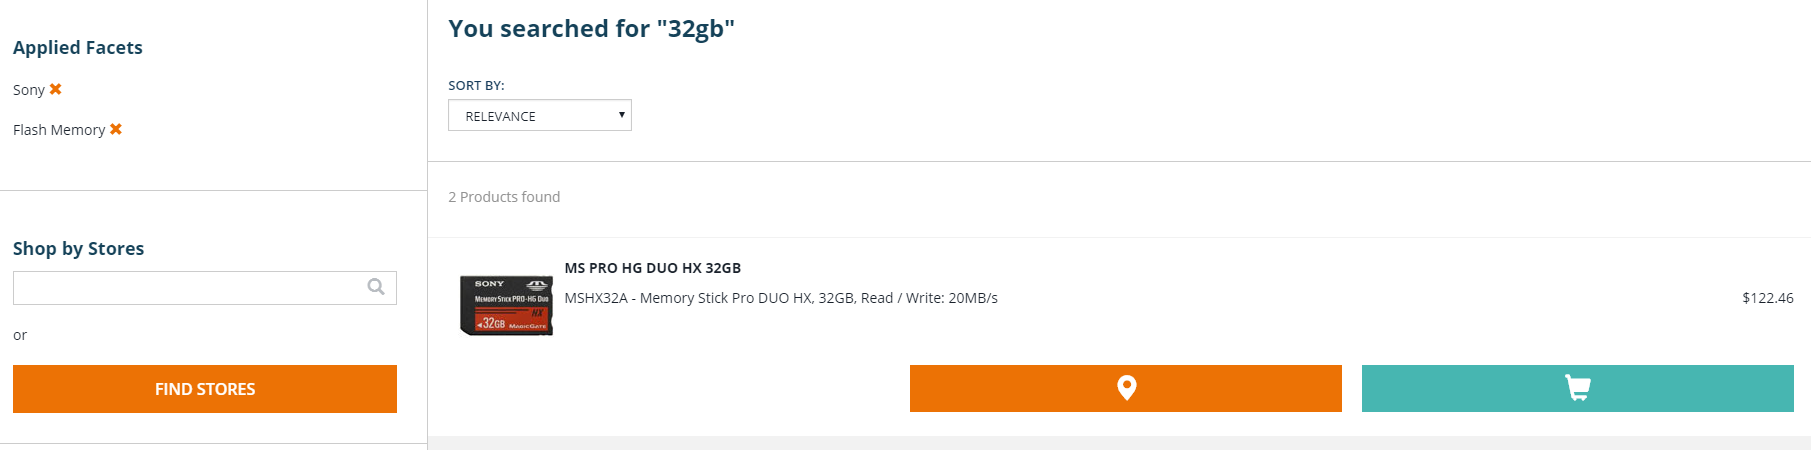
\includegraphics[width=\columnwidth]{2017-06-25_22h24_20-1.png}
        \caption{The system correctly applying multiple facets for the unambiguous query “Sony Flash memory 32Gb”.}
        \label{fig:unambiguous_query}
    \end{figure}

    To facilitate this mapping, the system retrieves all available facet values directly from the SOLR index using its built-in "terms" request handler. For optimal performance, this technique requires SOLR fields configured with a \texttt{KeywordTokenizer} and without stemming filters.

    \begin{figure}[H]
        \centering
        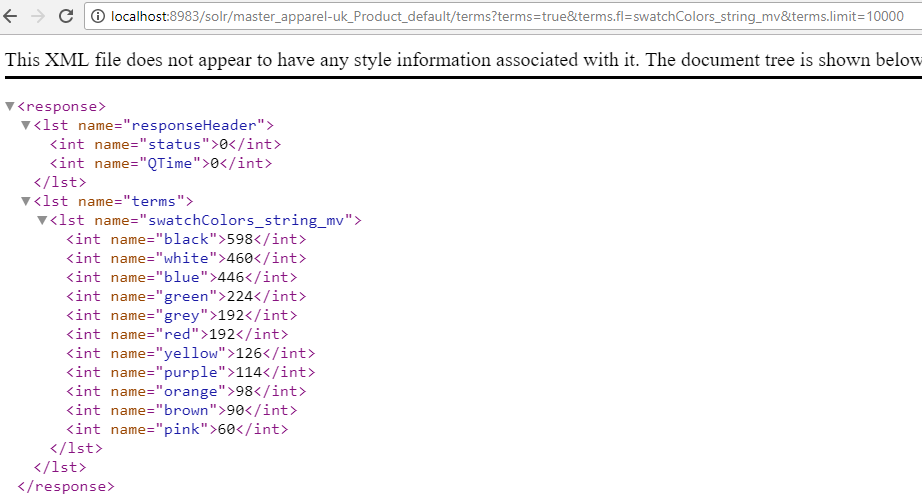
\includegraphics[width=\columnwidth]{2017-06-25_22h33_17-1.png}
        \caption{The SOLR terms component response, listing all values for a given facet field.}
        \label{fig:solr_terms}
    \end{figure}

    The PoC employs an efficient strategy by only processing facets that are returned by an initial standard keyword search.
    \begin{figure}[H]
        \centering
        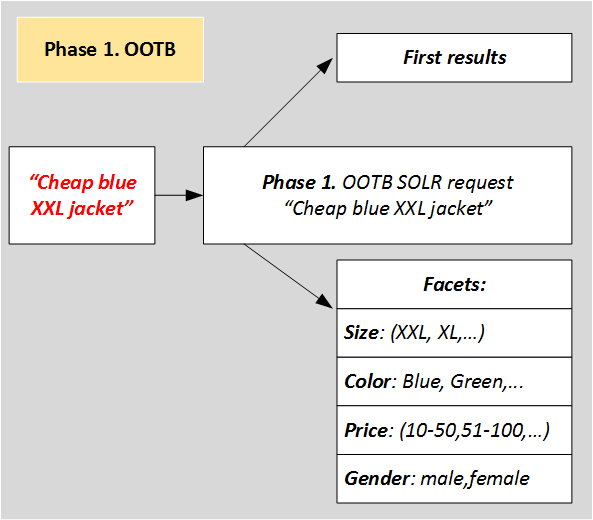
\includegraphics[width=0.8\columnwidth]{searchimproved2.png}
        \caption{Step 1: The system performs an initial full-text search to retrieve a set of relevant facets.}
        \label{fig:process_flow1}
    \end{figure}

    Once terms are mapped to facets, the remaining query words are categorized as stopwords, special commands, or residual keywords.
    \begin{figure}[H]
        \centering
        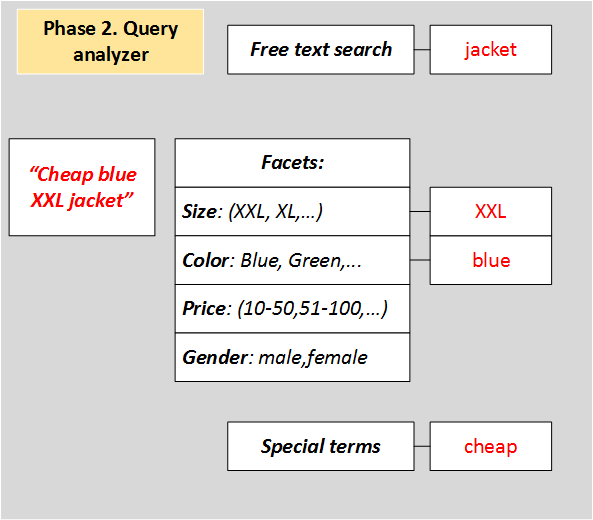
\includegraphics[width=0.8\columnwidth]{searchimproved3.png}
        \caption{Step 2: Query terms are mapped against the values of the retrieved facets.}
        \label{fig:process_flow2}
    \end{figure}

    The system then constructs a new, hybrid query combining the discovered facet filters with the remaining keywords.
    \begin{figure}[H]
        \centering
        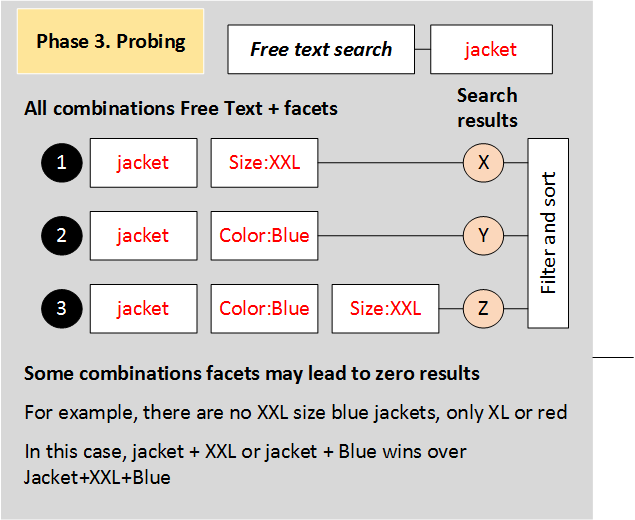
\includegraphics[width=0.8\columnwidth]{searchimproved4-1.png}
        \caption{Step 3: A new, hybrid query is constructed using the identified facets and remaining keywords.}
        \label{fig:process_flow3}
    \end{figure}

    To handle conflicts where a term matches multiple facets (e.g., "red" as a color vs. part of the brand "Red Hat"), the PoC implements a simple disambiguation logic: it executes a count for each interpretation and proceeds with the option that yields a non-zero result set.

    \section{Conclusion and Future Work}

    This paper has presented a proof-of-concept for an automatic facet discovery system. By programmatically parsing unstructured user queries to identify and apply corresponding structured facet filters, the proposed system effectively bridges the semantic gap between keyword-based retrieval and faceted navigation.

    The current implementation, while promising, has several recognized limitations. The system's reliance on exact-match string comparisons is inherently brittle. Furthermore, the conflict resolution logic is heuristic-based and could be substantially improved. The PoC does not yet support complex linguistic constructs.

    Future work will focus on integrating more sophisticated Natural Language Processing (NLP) techniques. The exploration of libraries such as OpenNLP is underway to incorporate capabilities like stemming and synonym expansion. Further research will also involve developing a more robust disambiguation model, potentially leveraging machine learning. Finally, a quantitative evaluation through rigorous A/B testing is required to measure the system's impact on key performance indicators. Ultimately, the continued development of such intelligent query interpretation systems is a critical step toward creating more intuitive and efficient information retrieval experiences.

\end{document}